% =====================================================================
%  Aprendizaje No Supervisado — Sesión 2: k-medias (k-means)
%  Unidad 1: Algoritmos de agrupamiento
%  Compilar con: latexmk -pdf Sesion2-KMedias.tex
%  Figuras: python3 figuras/generar_figuras.py
%  El laboratorio está en Laboratorio.tex (se incluye al final con \input)
% =====================================================================
\documentclass[aspectratio=169,11pt]{beamer}

\usepackage[utf8]{inputenc}
\usepackage[T1]{fontenc}
\usepackage[spanish,es-noshorthands,es-nodecimaldot]{babel}
\usepackage{amsmath,amssymb,bm}
\usepackage{booktabs,array}
\usepackage{listings}
\usepackage{tikz}
\usetikzlibrary{positioning,arrows.meta}
\graphicspath{{figuras/}}
\tikzset{caja/.style={draw=azul,fill=azul!10,rounded corners,align=center,font=\small,
  minimum height=9mm}}

% ---------- Tema (común a las presentaciones del curso) ----------
\usetheme{Madrid}
\usefonttheme{professionalfonts}
\definecolor{marino}{HTML}{1F3864}
\definecolor{azul}{HTML}{2E75B6}
\definecolor{naranja}{HTML}{E07B22}
\definecolor{verde}{HTML}{5B9A3C}
\definecolor{fondocod}{HTML}{F4F6F9}
\setbeamercolor{palette primary}{bg=marino,fg=white}
\setbeamercolor{palette secondary}{bg=azul,fg=white}
\setbeamercolor{palette tertiary}{bg=marino,fg=white}
\setbeamercolor{frametitle}{bg=marino,fg=white}
\setbeamercolor{title}{bg=marino,fg=white}
\setbeamercolor{structure}{fg=azul}
\setbeamercolor{block title}{bg=azul,fg=white}
\setbeamercolor{block body}{bg=azul!8}
\setbeamercolor{block title alerted}{bg=naranja,fg=white}
\setbeamercolor{block body alerted}{bg=naranja!10}
\setbeamercolor{block title example}{bg=verde,fg=white}
\setbeamercolor{block body example}{bg=verde!10}
\setbeamercolor{alerted text}{fg=naranja}
\setbeamertemplate{navigation symbols}{}
\setbeamertemplate{itemize items}[circle]
\setbeamertemplate{blocks}[rounded][shadow=false]

\AtBeginSection[]{
  \begin{frame}
    \vfill\centering
    \begin{beamercolorbox}[sep=12pt,center,rounded=true]{title}
      \usebeamerfont{title}\insertsectionhead
    \end{beamercolorbox}
    \vfill
  \end{frame}
}

\lstdefinestyle{py}{
  language=Python, basicstyle=\ttfamily\scriptsize,
  keywordstyle=\color{marino}\bfseries, commentstyle=\color{gray}\itshape,
  stringstyle=\color{naranja}, backgroundcolor=\color{fondocod},
  frame=single, rulecolor=\color{azul!40}, showstringspaces=false,
  columns=fullflexible, breaklines=true, xleftmargin=4pt, xrightmargin=4pt
}
\lstset{style=py}

\newcommand{\R}{\mathbb{R}}
\newcommand{\x}{\bm{x}}
\newcommand{\muv}{\bm{\mu}}

\title[Sesión 2: k-medias]{Sesión 2: k-medias (\emph{k-means})}
\subtitle{Aprendizaje No Supervisado --- Unidad 1: Algoritmos de agrupamiento}
\author[A. Espinosa Romero]{Arturo Espinosa Romero}
\institute[FMAT]{Maestría en Inteligencia Artificial \\ Facultad de Matemáticas}
\date{Sesión 2}

% =====================================================================
\begin{document}

\begin{frame}
  \titlepage
\end{frame}

\begin{frame}{Agenda de la sesión}
  \begin{columns}[T]
    \column{0.55\textwidth}
    \begin{enumerate}
      \item El problema del agrupamiento
      \item Función objetivo de k-medias (inercia)
      \item Algoritmo de Lloyd y su convergencia
      \item Inicialización k-means++ y múltiples reinicios
      \item Elección de $k$: codo y silueta
      \item Limitaciones: forma, escala y atípicos
      \item Laboratorio: k-medias con el conjunto Iris
    \end{enumerate}
    \column{0.4\textwidth}
    \begin{block}{Al terminar podrás}
      \begin{itemize}
        \item Explicar qué optimiza k-medias y por qué funciona Lloyd
        \item Aplicarlo con scikit-learn
        \item Elegir $k$ con criterios explícitos
        \item Reconocer cuándo \emph{no} usarlo
      \end{itemize}
    \end{block}
  \end{columns}
\end{frame}

% =====================================================================
\section{El problema del agrupamiento}
% =====================================================================

\begin{frame}{Problema detonador: ¿cuántos tipos de flores hay?}
  \begin{columns}[c]
    \column{0.55\textwidth}
    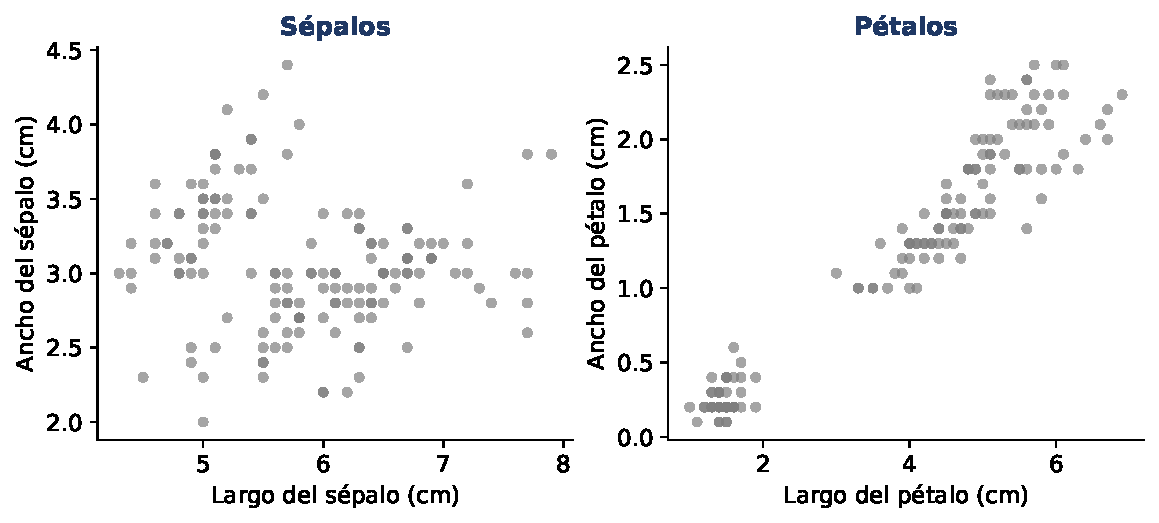
\includegraphics[width=\textwidth]{iris_detonador}
    \column{0.42\textwidth}
    Conjunto \textbf{Iris} (Fisher, 1936): 150 flores con cuatro medidas en centímetros,
    largo y ancho del sépalo y del pétalo.
    \vspace{4pt}
    \begin{alertblock}{Supongamos que no conocemos la especie}
      \begin{itemize}
        \item ¿Las medidas forman grupos naturales?
        \item ¿Cuántos?
        \item ¿Qué distingue a cada grupo?
      \end{itemize}
    \end{alertblock}
  \end{columns}
  \vspace{4pt}
  {\small La especie sí está registrada (setosa, versicolor, virginica): no la usaremos para
  agrupar, sólo para evaluar al final. En \texttt{scikit-learn}: \texttt{sklearn.datasets.load\_iris}.}
\end{frame}

\begin{frame}{¿Qué es agrupar?}
  Dado $\{\x_1,\dots,\x_n\}\subset\R^d$, encontrar una partición en $k$ grupos
  $C_1,\dots,C_k$ tal que:
  \begin{itemize}
    \item los objetos de un mismo grupo sean \alert{parecidos} entre sí, y
    \item los de grupos distintos sean \alert{diferentes}.
  \end{itemize}
  \vspace{6pt}
  \begin{block}{k-medias concreta ``parecido''}
    Cada grupo se representa con un \textbf{centro} (prototipo) $\muv_j$, y un objeto
    pertenece al grupo cuyo centro está más cerca en \textbf{distancia euclidiana}.
  \end{block}
  \vspace{4pt}
  {\small Recordatorio de la Sesión 1: la distancia euclidiana depende de la escala;
  hay que estandarizar cuando las unidades difieren.}
\end{frame}

% =====================================================================
\section{Función objetivo}
% =====================================================================

\begin{frame}{Inercia: suma de cuadrados dentro de los grupos}
  Buscar centros $\muv_1,\dots,\muv_k$ y asignaciones $z_i\in\{1,\dots,k\}$ que minimicen
  \[
    J(z,\muv) = \sum_{i=1}^{n} \lVert \x_i - \muv_{z_i} \rVert^2
      = \sum_{j=1}^{k}\sum_{i\in C_j} \lVert \x_i - \muv_j \rVert^2 .
  \]
  Para un grupo fijo, la inercia equivale a las diferencias entre todos sus pares de puntos:
  \[
    \sum_{i\in C_j}\lVert\x_i-\muv_j\rVert^2 = \frac{1}{2\,n_j}\sum_{i\in C_j}\sum_{i'\in C_j}\lVert\x_i-\x_{i'}\rVert^2 ,
    \qquad n_j = |C_j| .
  \]
  {\small Minimizar $J$ es buscar grupos internamente compactos (James et al., 2023, ec.~12.17).}
\end{frame}

\begin{frame}{Dentro y entre grupos}
  Con $\bar{\x}$ la media global, la dispersión total se descompone (teorema de Huygens):
  \[
    \underbrace{\sum_{i=1}^n\lVert\x_i-\bar{\x}\rVert^2}_{T\ \text{(total, fija)}}
    = \underbrace{\sum_{j=1}^k\sum_{i\in C_j}\lVert\x_i-\muv_j\rVert^2}_{W = J\ \text{(dentro)}}
    + \underbrace{\sum_{j=1}^k n_j\,\lVert\muv_j-\bar{\x}\rVert^2}_{B\ \text{(entre)}} .
  \]
  \begin{itemize}
    \item Como $T$ no depende de la partición, \alert{minimizar $W$ equivale a maximizar $B$}:
          grupos compactos y, a la vez, separados.
    \item Encontrar el mínimo global de $J$ es NP-difícil, incluso con $k=2$.
    \item Número de particiones posibles: crece aproximadamente como $k^n/k!$.
  \end{itemize}
\end{frame}

\begin{frame}{Dos subproblemas fáciles}
  \begin{columns}[T]
    \column{0.48\textwidth}
    \begin{block}{Centros fijos $\Rightarrow$ asignación óptima}
      Cada punto va al centro más cercano:
      \[ z_i = \arg\min_{j}\lVert\x_i-\muv_j\rVert^2 . \]
    \end{block}
    \column{0.48\textwidth}
    \begin{block}{Asignación fija $\Rightarrow$ centros óptimos}
      Derivando $\sum_{i\in C_j}\lVert\x_i-\muv_j\rVert^2$:
      \[ -2\sum_{i\in C_j}(\x_i-\muv_j) = 0
         \;\Rightarrow\;
         \muv_j = \frac{1}{n_j}\sum_{i\in C_j}\x_i . \]
    \end{block}
  \end{columns}
  \vspace{8pt}
  \begin{alertblock}{Idea del algoritmo}
    Alternar ambos pasos. Cada uno minimiza $J$ respecto a una parte de las variables:
    es un \textbf{descenso por coordenadas}. De ahí el nombre: los centros son \emph{medias}.
  \end{alertblock}
\end{frame}

% =====================================================================
\section{Algoritmo de Lloyd}
% =====================================================================

\begin{frame}{Algoritmo de Lloyd}
  \centering
  \begin{tikzpicture}[node distance=6mm,every node/.append style={font=\footnotesize}]
    \node[caja] (i) {Inicializar\\$\muv_1,\dots,\muv_k$};
    \node[caja,right=of i] (a) {\textbf{Asignación}\\$z_i\leftarrow\arg\min_j\lVert\x_i-\muv_j\rVert^2$};
    \node[caja,right=of a] (u) {\textbf{Actualización}\\$\muv_j\leftarrow$ media de $C_j$};
    \node[caja,draw=naranja,fill=naranja!12,right=of u] (f) {¿Cambió\\alguna $z_i$?};
    \draw[-{Stealth},thick,marino] (i) -- (a);
    \draw[-{Stealth},thick,marino] (a) -- (u);
    \draw[-{Stealth},thick,marino] (u) -- (f);
    \draw[-{Stealth},thick,marino] (f.south) -- ++(0,-0.6) -| node[pos=0.25,below,font=\scriptsize]{sí} (a.south);
    \node[above=1mm of f,font=\scriptsize] {no: fin};
  \end{tikzpicture}
  \vspace{2pt}
  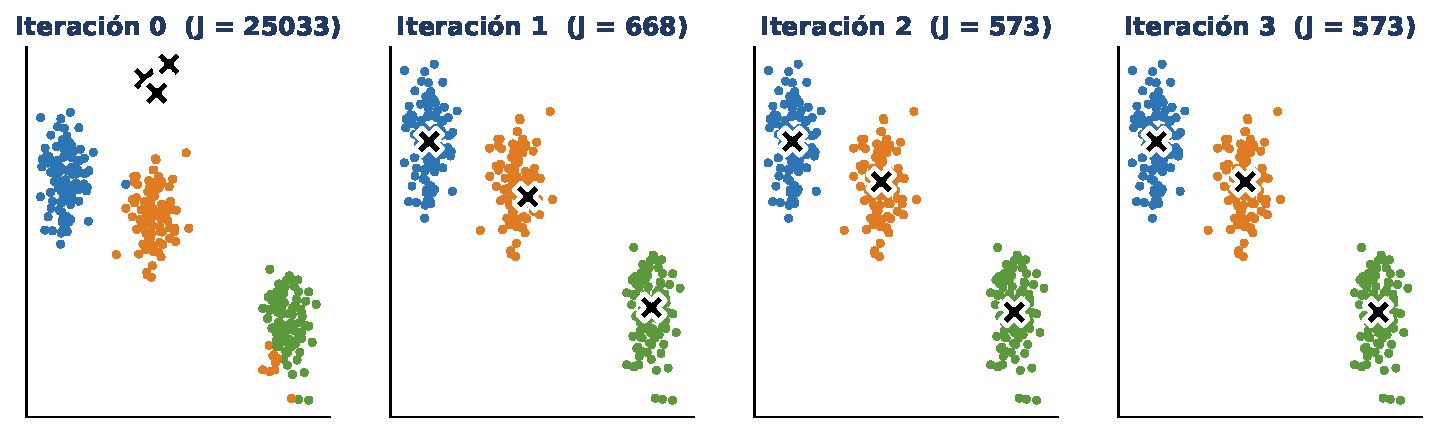
\includegraphics[width=0.88\textwidth]{lloyd_iteraciones}\\
  {\small Desde una mala inicialización (cruces arriba), Lloyd se recupera en dos iteraciones.}
\end{frame}

\begin{frame}{Regiones de asignación}
  \begin{columns}[c]
    \column{0.45\textwidth}
    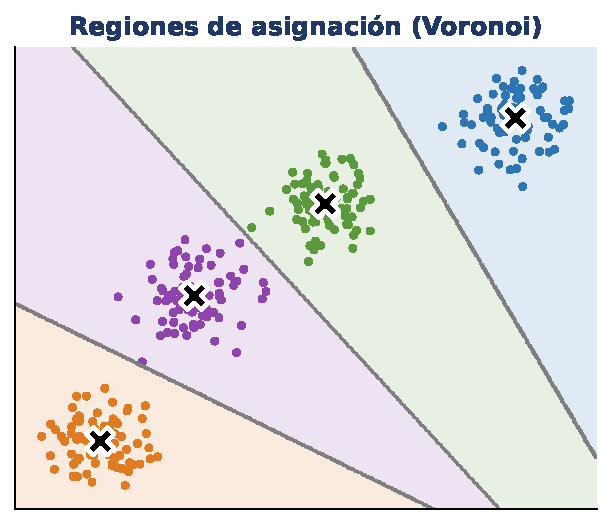
\includegraphics[width=\textwidth]{voronoi}
    \column{0.52\textwidth}
    \begin{itemize}
      \item Cada centro ``captura'' la región del espacio más cercana a él: una \textbf{celda de Voronoi}.
      \item La frontera entre dos centros es el \alert{hiperplano mediador} del segmento que los une.
      \item Por eso k-medias sólo produce grupos \textbf{convexos}, separados por fronteras lineales.
      \item Un punto nuevo se asigna con el mismo criterio: \texttt{predict}.
    \end{itemize}
  \end{columns}
\end{frame}

\begin{frame}{Convergencia y costo}
  \begin{block}{¿Por qué termina?}
    \begin{itemize}
      \item Ningún paso aumenta $J$: cada uno es óptimo para su subproblema.
      \item Hay un número finito de particiones y ninguna se repite mientras $J$ baje.
      \item Por lo tanto, Lloyd converge en un número finito de iteraciones.
    \end{itemize}
  \end{block}
  \begin{alertblock}{Pero\dots}
    Converge a un \textbf{mínimo local}, que depende de la inicialización.
  \end{alertblock}
  \begin{itemize}
    \item Costo por iteración: $O(nkd)$; en la práctica bastan pocas decenas de iteraciones.
    \item Variante de Elkan: usa la desigualdad del triángulo para evitar calcular distancias innecesarias.
  \end{itemize}
\end{frame}

\begin{frame}{Ejemplo: un mínimo local en una dimensión}
  Datos $x = \{1,\ 2,\ 3,\ 8,\ 9,\ 10,\ 25\}$, $k=2$, centros iniciales $\mu_1 = 1$, $\mu_2 = 2$.
  \vspace{4pt}
  \begin{center}
    \renewcommand{\arraystretch}{1.2}
    \begin{tabular}{@{}llll@{}}
      \toprule
      \textbf{Iteración} & \textbf{Centros} & \textbf{Grupos} & $J$\\
      \midrule
      0 & $1,\ 2$ & $\{1\}$, $\{2,3,8,9,10,25\}$ & 679 \\
      1 & $1,\ 9.5$ & $\{1,2,3\}$, $\{8,9,10,25\}$ & 248 \\
      2 & $2,\ 13$ & $\{1,2,3\}$, $\{8,9,10,25\}$ & 196 \\
      \bottomrule
    \end{tabular}
  \end{center}
  \begin{itemize}
    \item En la iteración 2 las asignaciones ya no cambian: Lloyd se detiene con $J = 196$.
    \item La partición $\{1,2,3,8,9,10\}$, $\{25\}$ tiene $J = 77.5$: Lloyd quedó en un \alert{mínimo local}.
    \item Ese óptimo global dedica un grupo completo al \alert{atípico} 25.
  \end{itemize}
\end{frame}

% =====================================================================
\section{Inicialización}
% =====================================================================

\begin{frame}{Estrategias de inicialización}
  \begin{itemize}
    \item \textbf{Aleatoria (Forgy)}: elegir $k$ observaciones al azar como centros.
    \item \textbf{Partición aleatoria}: asignar cada punto a un grupo al azar y calcular medias.
    \item \textbf{k-means++} (Arthur y Vassilvitskii, 2007): centros iniciales \alert{dispersos}.
  \end{itemize}
  \vspace{4pt}
  \begin{block}{k-means++}
    \begin{enumerate}
      \item Elegir el primer centro uniformemente entre los datos.
      \item Para cada punto, $D(\x)$ = distancia al centro ya elegido más cercano.
      \item Elegir el siguiente centro con probabilidad
            $\displaystyle P(\x_i) = \frac{D(\x_i)^2}{\sum_l D(\x_l)^2}$.
      \item Repetir 2--3 hasta tener $k$ centros; luego ejecutar Lloyd.
    \end{enumerate}
  \end{block}
  {\small Garantía: en esperanza, la inercia inicial es a lo más $O(\log k)$ veces la óptima.}
\end{frame}

\begin{frame}{Múltiples reinicios}
  \begin{columns}[c]
    \column{0.52\textwidth}
    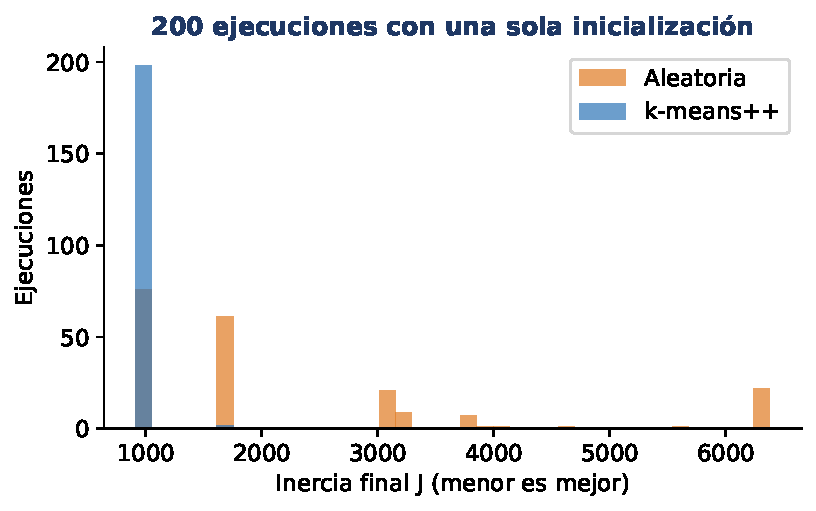
\includegraphics[width=\textwidth]{inicializacion}
    \column{0.45\textwidth}
    \begin{itemize}
      \item 8 grupos bien separados, 200 ejecuciones con una sola inicialización.
      \item Con inicialización aleatoria, muchas ejecuciones terminan con $J$ alto.
      \item k-means++ reduce mucho la variabilidad, pero no la elimina.
    \end{itemize}
    \begin{alertblock}{Práctica recomendada}
      Varios reinicios (\texttt{n\_init}) y quedarse con la solución de menor $J$.
    \end{alertblock}
  \end{columns}
\end{frame}

% =====================================================================
\section{Elección de \texorpdfstring{$k$}{k}}
% =====================================================================

\begin{frame}{Método del codo}
  \begin{columns}[c]
    \column{0.55\textwidth}
    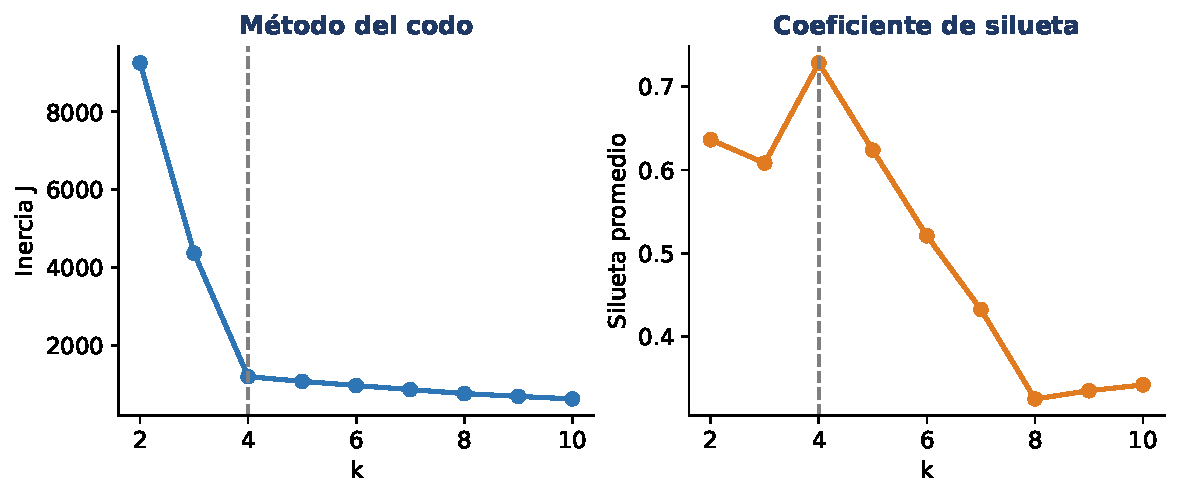
\includegraphics[width=\textwidth]{codo_silueta}
    \column{0.42\textwidth}
    \begin{itemize}
      \item $J$ \alert{siempre} disminuye al aumentar $k$ (con $k=n$, $J=0$).
      \item No se puede elegir $k$ minimizando $J$.
      \item \textbf{Codo}: el $k$ a partir del cual la mejora se vuelve marginal.
      \item Con datos reales el codo suele ser ambiguo.
    \end{itemize}
  \end{columns}
\end{frame}

\begin{frame}{Coeficiente de silueta}
  Para cada punto $i$ de un grupo $C$:
  \begin{itemize}
    \item $a(i)$: distancia media de $i$ a los demás puntos de $C$ (cohesión).
    \item $b(i)$: menor distancia media de $i$ a los puntos de otro grupo (separación).
  \end{itemize}
  \[
    s(i) = \frac{b(i)-a(i)}{\max\{a(i),\,b(i)\}} \in [-1, 1]
  \]
  \begin{columns}[T]
    \column{0.48\textwidth}
    \begin{itemize}
      \item $s(i)\approx 1$: bien asignado.
      \item $s(i)\approx 0$: en la frontera.
      \item $s(i)<0$: probablemente mal asignado.
    \end{itemize}
    \column{0.48\textwidth}
    \begin{block}{Criterio}
      Elegir el $k$ con mayor silueta promedio (Rousseeuw, 1987).
    \end{block}
  \end{columns}
\end{frame}

\begin{frame}{Diagrama de silueta}
  \centering
  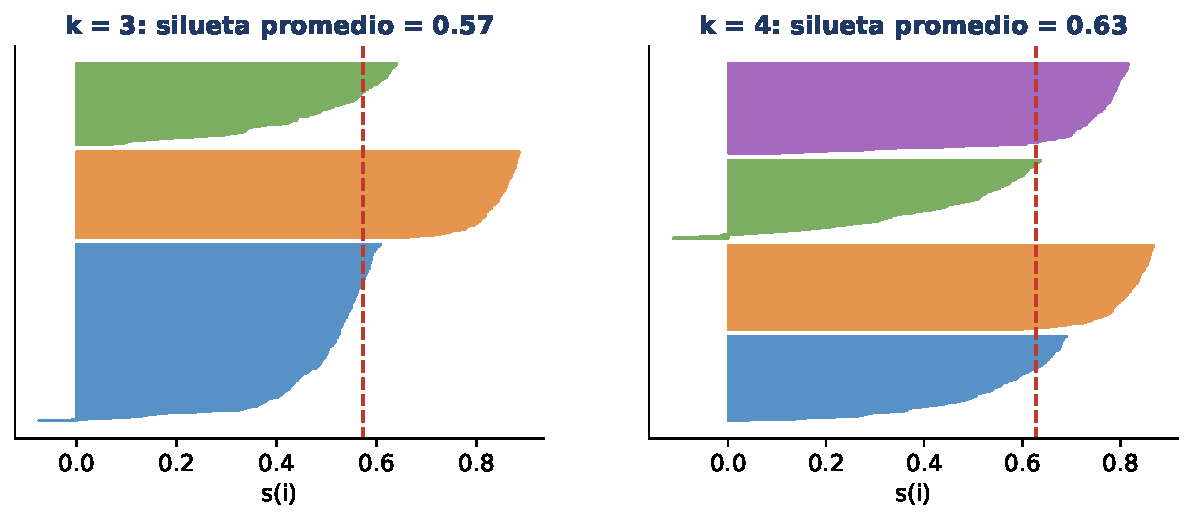
\includegraphics[width=0.72\textwidth]{diagrama_silueta}
  \begin{itemize}
    \item Cada franja horizontal es un punto; cada color, un grupo.
    \item Además del promedio, revisar que todos los grupos superen la media y no tengan valores negativos.
    \item Otros criterios: estadístico \emph{gap} (Tibshirani et al., 2001) e índices que veremos en la Sesión 6.
  \end{itemize}
\end{frame}

\begin{frame}{$k$ también es una decisión del problema}
  \begin{itemize}
    \item Los criterios numéricos orientan, pero no deciden solos.
    \item ¿Cuántos segmentos puede atender el área comercial? ¿Tres campañas o diez?
    \item Un grupo debe ser \alert{interpretable} y \alert{accionable}.
    \item Comparar soluciones con $k$ cercanos: ¿se divide un grupo con sentido o se fragmenta ruido?
  \end{itemize}
  \vspace{6pt}
  \begin{block}{Lo veremos con Iris}
    La silueta favorece $k=2$, aunque hay tres especies: dos de ellas se traslapan.
  \end{block}
\end{frame}

% =====================================================================
\section{Limitaciones}
% =====================================================================

\begin{frame}{Supuestos implícitos}
  \centering
  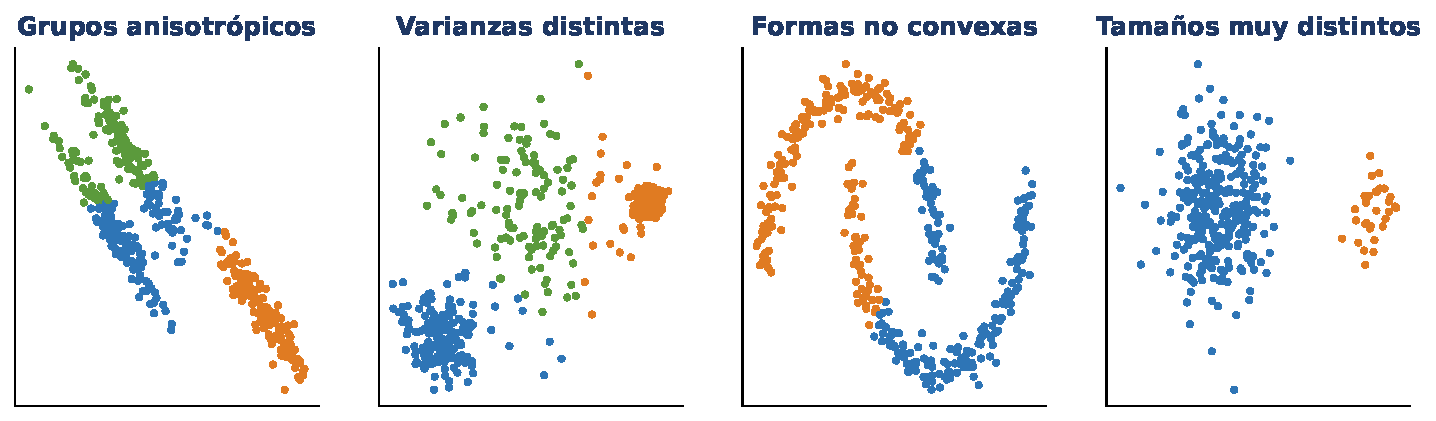
\includegraphics[width=\textwidth]{limitaciones}
  \begin{columns}[T]
    \column{0.48\textwidth}
    \begin{itemize}
      \item Grupos \alert{esféricos} (isotrópicos).
      \item Varianzas parecidas entre grupos.
    \end{itemize}
    \column{0.48\textwidth}
    \begin{itemize}
      \item Grupos \alert{convexos}.
      \item Tamaños comparables: tiende a partir los grupos grandes.
    \end{itemize}
  \end{columns}
\end{frame}

\begin{frame}{Escala y valores atípicos}
  \begin{columns}[c]
    \column{0.55\textwidth}
    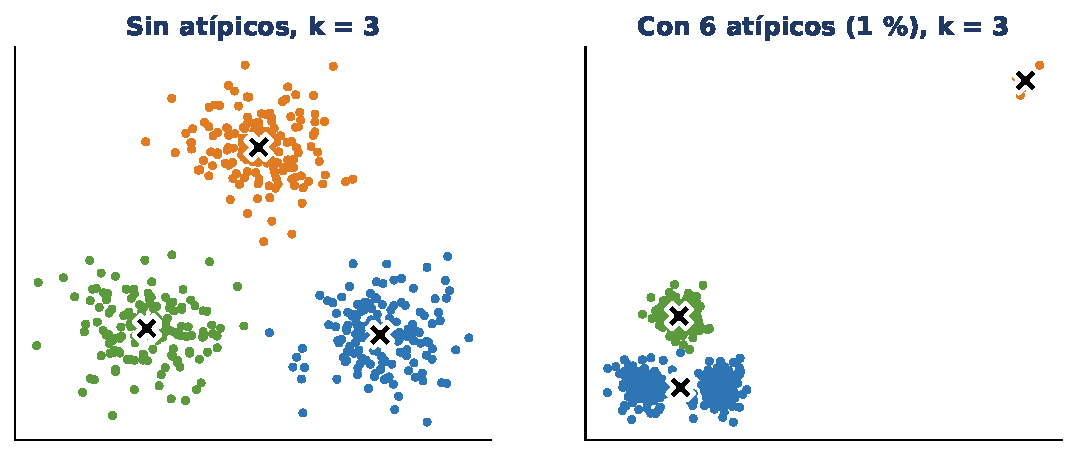
\includegraphics[width=\textwidth]{atipicos}
    \column{0.42\textwidth}
    \begin{itemize}
      \item Seis puntos lejanos (1\,\% de los datos) se llevan un centro completo y dos grupos reales se fusionan.
      \item La media y el error cuadrático amplifican los valores extremos.
      \item La variable con mayor escala domina la distancia (Sesión 1).
    \end{itemize}
  \end{columns}
  \vspace{4pt}
  \begin{block}{Remedios}
    Estandarizar; transformar variables sesgadas (logaritmo); revisar atípicos antes de agrupar;
    usar variantes robustas.
  \end{block}
\end{frame}

\begin{frame}{Variantes}
  \renewcommand{\arraystretch}{1.3}
  \begin{tabular}{@{}>{\raggedright\arraybackslash}p{0.24\textwidth}>{\raggedright\arraybackslash}p{0.4\textwidth}>{\raggedright\arraybackslash}p{0.28\textwidth}@{}}
    \toprule
    \textbf{Variante} & \textbf{Idea} & \textbf{Cuándo usarla}\\
    \midrule
    k-medoides (PAM) & Centros restringidos a observaciones; admite cualquier distancia & Atípicos, distancias no euclidianas \\
    k-medianas & Mediana por coordenada y distancia $\ell_1$ & Robustez \\
    Mini-batch k-medias & Actualiza los centros con lotes pequeños & $n$ muy grande \\
    k-modos / k-prototipos & Modas para variables categóricas & Datos categóricos o mixtos \\
    \bottomrule
  \end{tabular}
  \vspace{6pt}
  {\small Las limitaciones de forma las resuelven otros algoritmos de la unidad:
  mezclas gaussianas (S4) y métodos por densidad y espectrales (S5).}
\end{frame}

\begin{frame}[fragile]{k-medias en scikit-learn}
\begin{lstlisting}
from sklearn.cluster import KMeans

km = KMeans(
    n_clusters=4,        # k
    init="k-means++",    # o "random", o un arreglo con centros iniciales
    n_init=10,           # reinicios; se conserva el de menor inercia
    max_iter=300, tol=1e-4,
    algorithm="lloyd",   # o "elkan"
    random_state=0,
).fit(X)

km.labels_            # asignacion z_i de cada punto
km.cluster_centers_   # centros (k x d)
km.inertia_           # J final
km.n_iter_            # iteraciones de Lloyd
km.predict(X_nuevo)   # asignar puntos nuevos al centro mas cercano
km.transform(X)       # distancias de cada punto a cada centro (n x k)
\end{lstlisting}
\end{frame}

% =====================================================================
%  Laboratorio (para omitirlo de las láminas, comentar la línea siguiente)
% =====================================================================
%  Laboratorio de la Sesión 2: k-medias con el conjunto Iris
%  Se incluye desde Sesion2-KMedias.tex con % =====================================================================
%  Laboratorio de la Sesión 2: k-medias con el conjunto Iris
%  Se incluye desde Sesion2-KMedias.tex con % =====================================================================
%  Laboratorio de la Sesión 2: k-medias con el conjunto Iris
%  Se incluye desde Sesion2-KMedias.tex con \input{Laboratorio}
% =====================================================================
\section{Laboratorio: k-medias con Iris}
% =====================================================================

\begin{frame}[fragile]{Paso 1: cargar y explorar los datos}
\begin{lstlisting}
import numpy as np, pandas as pd
from sklearn.datasets import load_iris

iris = load_iris(as_frame=True)
X = iris.data                  # 150 x 4, medidas en cm
especie = iris.target          # se guarda aparte: NO se usa para agrupar

print(X.describe().T[["mean", "std", "min", "max"]])
\end{lstlisting}
  \vspace{2pt}
  \centering
  \small
  \begin{tabular}{@{}lcccc@{}}
    \toprule
    \textbf{Variable (cm)} & \textbf{Media} & \textbf{Desv.\ est.} & \textbf{Mín.} & \textbf{Máx.}\\
    \midrule
    Largo del sépalo & 5.84 & 0.83 & 4.3 & 7.9 \\
    Ancho del sépalo & 3.06 & 0.44 & 2.0 & 4.4 \\
    Largo del pétalo & 3.76 & 1.77 & 1.0 & 6.9 \\
    Ancho del pétalo & 1.20 & 0.76 & 0.1 & 2.5 \\
    \bottomrule
  \end{tabular}\\[4pt]
  \raggedright
  {\small Las cuatro variables están en la misma unidad. Los pétalos tienen la mayor variación.}
\end{frame}

\begin{frame}[fragile]{Paso 2: elegir $k$}
\begin{lstlisting}
from sklearn.cluster import KMeans
from sklearn.metrics import silhouette_score

for k in range(2, 9):
    km = KMeans(n_clusters=k, n_init=10, random_state=0).fit(X)
    print(k, round(km.inertia_, 1), round(silhouette_score(X, km.labels_), 3))
\end{lstlisting}
  \centering
  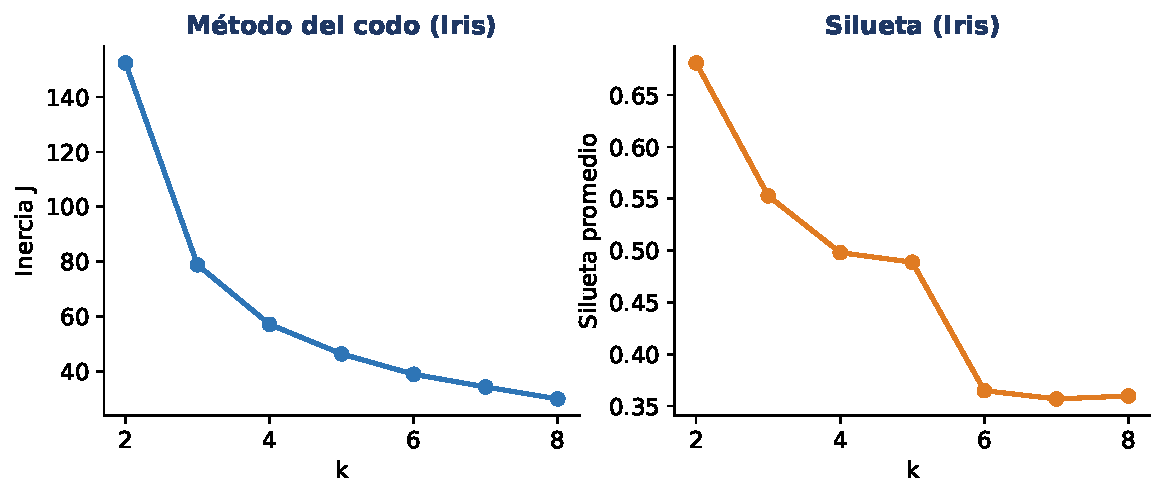
\includegraphics[width=0.62\textwidth]{iris_codo_silueta}\\
  \raggedright
  {\small El codo aparece entre $k=2$ y $k=3$. La silueta es máxima con $k=2$ (0.68) y baja a 0.55 con $k=3$.}
\end{frame}

\begin{frame}{Paso 2: ¿dos o tres grupos?}
  \begin{itemize}
    \item Los criterios numéricos sugieren $k=2$: una especie (setosa) está muy separada
          y las otras dos se traslapan.
    \item Con $k=3$ el codo todavía muestra una reducción importante de $J$ (de 152 a 79).
    \item Sabemos por el dominio que esperamos tres tipos de flor: elegimos $k=3$.
  \end{itemize}
  \vspace{6pt}
  \begin{alertblock}{Lección}
    La silueta mide qué tan separados quedan los grupos, no si corresponden a categorías reales.
    La elección de $k$ combina criterios numéricos y conocimiento del problema.
  \end{alertblock}
\end{frame}

\begin{frame}[fragile]{Paso 3: ajustar e interpretar los centros}
\begin{lstlisting}
km = KMeans(n_clusters=3, n_init=10, random_state=0).fit(X)
centros = pd.DataFrame(km.cluster_centers_, columns=X.columns)
print(centros.round(2)); print(np.bincount(km.labels_))
\end{lstlisting}
  \vspace{2pt}
  \centering
  \small
  \begin{tabular}{@{}lccccc@{}}
    \toprule
    \textbf{Grupo} & \textbf{Largo sépalo} & \textbf{Ancho sépalo} & \textbf{Largo pétalo} & \textbf{Ancho pétalo} & \textbf{Flores}\\
    \midrule
    A & 5.01 & 3.43 & 1.46 & 0.25 & 50 \\
    B & 5.90 & 2.75 & 4.39 & 1.43 & 62 \\
    C & 6.85 & 3.07 & 5.74 & 2.07 & 38 \\
    \bottomrule
  \end{tabular}\\[6pt]
  \raggedright
  \begin{itemize}
    \item Grupo A: pétalos pequeños y sépalos anchos.
    \item Grupos B y C: pétalos medianos y grandes, respectivamente.
  \end{itemize}
  {\small Los centros están en centímetros: se interpretan directamente como una flor ``típica'' de cada grupo.}
\end{frame}

\begin{frame}[fragile]{Paso 4: comparar con las especies}
\begin{lstlisting}
from sklearn.metrics import adjusted_rand_score
print(pd.crosstab(km.labels_, iris.target_names[especie]))
print(adjusted_rand_score(especie, km.labels_))   # 1 = coincidencia perfecta (S6)
\end{lstlisting}
  \begin{columns}[c]
    \column{0.58\textwidth}
    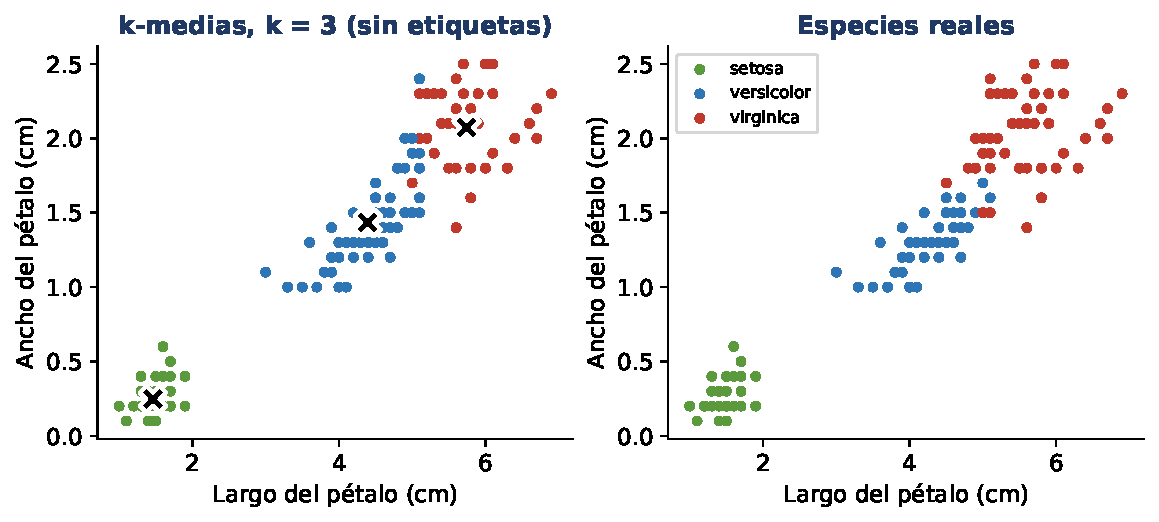
\includegraphics[width=\textwidth]{iris_resultado}
    \column{0.4\textwidth}
    \small
    \begin{tabular}{@{}lccc@{}}
      \toprule
      & \textbf{setosa} & \textbf{versic.} & \textbf{virgin.}\\
      \midrule
      A & 50 & 0 & 0 \\
      B & 0 & 48 & 14 \\
      C & 0 & 2 & 36 \\
      \bottomrule
    \end{tabular}\\[4pt]
    \begin{itemize}
      \item Setosa se recupera sin errores.
      \item 16 flores quedan en la frontera entre versicolor y virginica.
      \item Índice de Rand ajustado: 0.73.
    \end{itemize}
  \end{columns}
\end{frame}

\begin{frame}[fragile]{Paso 5: ¿conviene estandarizar?}
\begin{lstlisting}
from sklearn.pipeline import make_pipeline
from sklearn.preprocessing import StandardScaler

km_std = make_pipeline(StandardScaler(), KMeans(n_clusters=3, n_init=10, random_state=0))
etiquetas_std = km_std.fit_predict(X)
print(adjusted_rand_score(especie, etiquetas_std))
\end{lstlisting}
  \centering
  \small
  \begin{tabular}{@{}lcc@{}}
    \toprule
    \textbf{Datos ($k=3$)} & \textbf{Silueta} & \textbf{Rand ajustado}\\
    \midrule
    En centímetros & 0.55 & 0.73 \\
    Estandarizados & 0.46 & 0.62 \\
    \bottomrule
  \end{tabular}\\[6pt]
  \raggedright
  \begin{itemize}
    \item Aquí todas las variables tienen la misma unidad: estandarizar \alert{no es necesario}.
    \item Al estandarizar, el ancho del sépalo pesa lo mismo que los pétalos, que son más
          informativos, y el resultado empeora.
    \item Estandarizar es la regla cuando las unidades difieren (Sesión 1); no es automático.
  \end{itemize}
\end{frame}

\begin{frame}{Conclusiones del laboratorio}
  \begin{itemize}
    \item Sin usar la especie, k-medias descubre la estructura principal de Iris:
          un grupo bien separado y dos que se traslapan.
    \item Los criterios numéricos (silueta) sugieren $k=2$; el conocimiento del dominio lleva a $k=3$.
    \item Los centros, en las unidades originales, permiten describir cada grupo.
    \item Las decisiones de preprocesamiento cambian el resultado: deben justificarse.
    \item Las flores mal asignadas están en la frontera entre especies parecidas:
          k-medias asigna cada punto a un solo grupo, sin expresar incertidumbre
          (lo resolverán las mezclas gaussianas, Sesión 4).
  \end{itemize}
\end{frame}

% =====================================================================
\section{Laboratorio: k-medias con Iris}
% =====================================================================

\begin{frame}[fragile]{Paso 1: cargar y explorar los datos}
\begin{lstlisting}
import numpy as np, pandas as pd
from sklearn.datasets import load_iris

iris = load_iris(as_frame=True)
X = iris.data                  # 150 x 4, medidas en cm
especie = iris.target          # se guarda aparte: NO se usa para agrupar

print(X.describe().T[["mean", "std", "min", "max"]])
\end{lstlisting}
  \vspace{2pt}
  \centering
  \small
  \begin{tabular}{@{}lcccc@{}}
    \toprule
    \textbf{Variable (cm)} & \textbf{Media} & \textbf{Desv.\ est.} & \textbf{Mín.} & \textbf{Máx.}\\
    \midrule
    Largo del sépalo & 5.84 & 0.83 & 4.3 & 7.9 \\
    Ancho del sépalo & 3.06 & 0.44 & 2.0 & 4.4 \\
    Largo del pétalo & 3.76 & 1.77 & 1.0 & 6.9 \\
    Ancho del pétalo & 1.20 & 0.76 & 0.1 & 2.5 \\
    \bottomrule
  \end{tabular}\\[4pt]
  \raggedright
  {\small Las cuatro variables están en la misma unidad. Los pétalos tienen la mayor variación.}
\end{frame}

\begin{frame}[fragile]{Paso 2: elegir $k$}
\begin{lstlisting}
from sklearn.cluster import KMeans
from sklearn.metrics import silhouette_score

for k in range(2, 9):
    km = KMeans(n_clusters=k, n_init=10, random_state=0).fit(X)
    print(k, round(km.inertia_, 1), round(silhouette_score(X, km.labels_), 3))
\end{lstlisting}
  \centering
  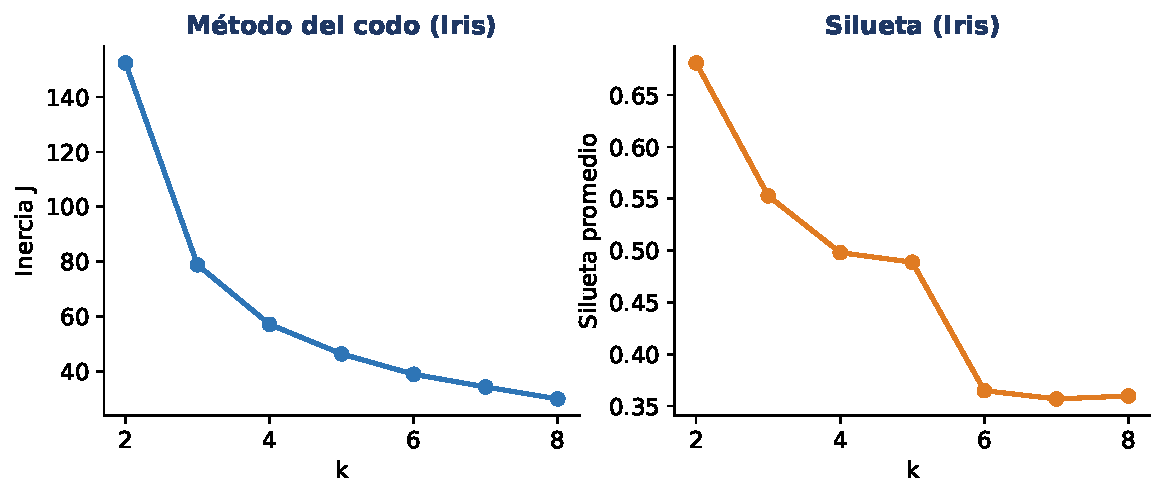
\includegraphics[width=0.62\textwidth]{iris_codo_silueta}\\
  \raggedright
  {\small El codo aparece entre $k=2$ y $k=3$. La silueta es máxima con $k=2$ (0.68) y baja a 0.55 con $k=3$.}
\end{frame}

\begin{frame}{Paso 2: ¿dos o tres grupos?}
  \begin{itemize}
    \item Los criterios numéricos sugieren $k=2$: una especie (setosa) está muy separada
          y las otras dos se traslapan.
    \item Con $k=3$ el codo todavía muestra una reducción importante de $J$ (de 152 a 79).
    \item Sabemos por el dominio que esperamos tres tipos de flor: elegimos $k=3$.
  \end{itemize}
  \vspace{6pt}
  \begin{alertblock}{Lección}
    La silueta mide qué tan separados quedan los grupos, no si corresponden a categorías reales.
    La elección de $k$ combina criterios numéricos y conocimiento del problema.
  \end{alertblock}
\end{frame}

\begin{frame}[fragile]{Paso 3: ajustar e interpretar los centros}
\begin{lstlisting}
km = KMeans(n_clusters=3, n_init=10, random_state=0).fit(X)
centros = pd.DataFrame(km.cluster_centers_, columns=X.columns)
print(centros.round(2)); print(np.bincount(km.labels_))
\end{lstlisting}
  \vspace{2pt}
  \centering
  \small
  \begin{tabular}{@{}lccccc@{}}
    \toprule
    \textbf{Grupo} & \textbf{Largo sépalo} & \textbf{Ancho sépalo} & \textbf{Largo pétalo} & \textbf{Ancho pétalo} & \textbf{Flores}\\
    \midrule
    A & 5.01 & 3.43 & 1.46 & 0.25 & 50 \\
    B & 5.90 & 2.75 & 4.39 & 1.43 & 62 \\
    C & 6.85 & 3.07 & 5.74 & 2.07 & 38 \\
    \bottomrule
  \end{tabular}\\[6pt]
  \raggedright
  \begin{itemize}
    \item Grupo A: pétalos pequeños y sépalos anchos.
    \item Grupos B y C: pétalos medianos y grandes, respectivamente.
  \end{itemize}
  {\small Los centros están en centímetros: se interpretan directamente como una flor ``típica'' de cada grupo.}
\end{frame}

\begin{frame}[fragile]{Paso 4: comparar con las especies}
\begin{lstlisting}
from sklearn.metrics import adjusted_rand_score
print(pd.crosstab(km.labels_, iris.target_names[especie]))
print(adjusted_rand_score(especie, km.labels_))   # 1 = coincidencia perfecta (S6)
\end{lstlisting}
  \begin{columns}[c]
    \column{0.58\textwidth}
    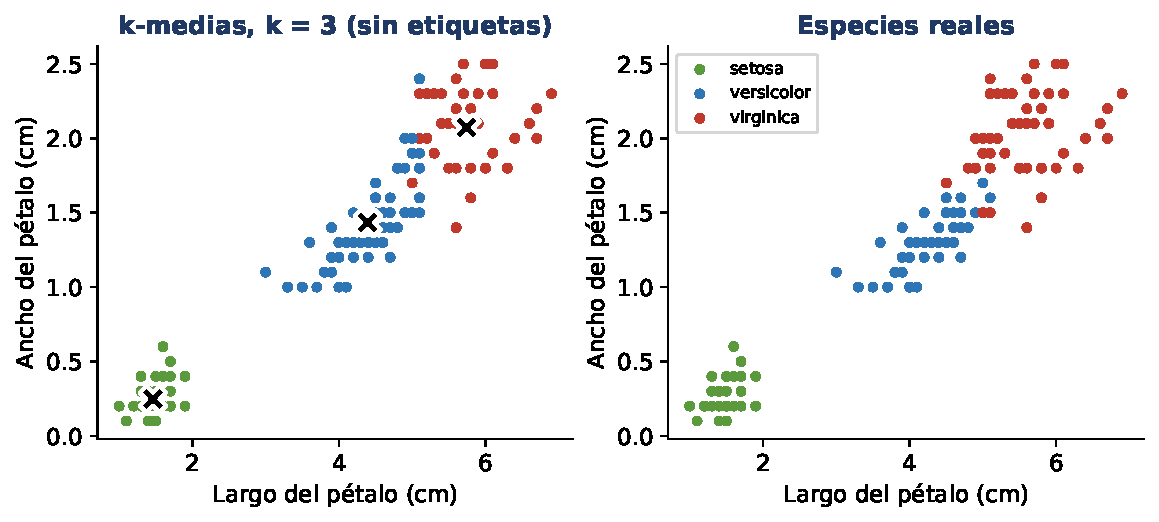
\includegraphics[width=\textwidth]{iris_resultado}
    \column{0.4\textwidth}
    \small
    \begin{tabular}{@{}lccc@{}}
      \toprule
      & \textbf{setosa} & \textbf{versic.} & \textbf{virgin.}\\
      \midrule
      A & 50 & 0 & 0 \\
      B & 0 & 48 & 14 \\
      C & 0 & 2 & 36 \\
      \bottomrule
    \end{tabular}\\[4pt]
    \begin{itemize}
      \item Setosa se recupera sin errores.
      \item 16 flores quedan en la frontera entre versicolor y virginica.
      \item Índice de Rand ajustado: 0.73.
    \end{itemize}
  \end{columns}
\end{frame}

\begin{frame}[fragile]{Paso 5: ¿conviene estandarizar?}
\begin{lstlisting}
from sklearn.pipeline import make_pipeline
from sklearn.preprocessing import StandardScaler

km_std = make_pipeline(StandardScaler(), KMeans(n_clusters=3, n_init=10, random_state=0))
etiquetas_std = km_std.fit_predict(X)
print(adjusted_rand_score(especie, etiquetas_std))
\end{lstlisting}
  \centering
  \small
  \begin{tabular}{@{}lcc@{}}
    \toprule
    \textbf{Datos ($k=3$)} & \textbf{Silueta} & \textbf{Rand ajustado}\\
    \midrule
    En centímetros & 0.55 & 0.73 \\
    Estandarizados & 0.46 & 0.62 \\
    \bottomrule
  \end{tabular}\\[6pt]
  \raggedright
  \begin{itemize}
    \item Aquí todas las variables tienen la misma unidad: estandarizar \alert{no es necesario}.
    \item Al estandarizar, el ancho del sépalo pesa lo mismo que los pétalos, que son más
          informativos, y el resultado empeora.
    \item Estandarizar es la regla cuando las unidades difieren (Sesión 1); no es automático.
  \end{itemize}
\end{frame}

\begin{frame}{Conclusiones del laboratorio}
  \begin{itemize}
    \item Sin usar la especie, k-medias descubre la estructura principal de Iris:
          un grupo bien separado y dos que se traslapan.
    \item Los criterios numéricos (silueta) sugieren $k=2$; el conocimiento del dominio lleva a $k=3$.
    \item Los centros, en las unidades originales, permiten describir cada grupo.
    \item Las decisiones de preprocesamiento cambian el resultado: deben justificarse.
    \item Las flores mal asignadas están en la frontera entre especies parecidas:
          k-medias asigna cada punto a un solo grupo, sin expresar incertidumbre
          (lo resolverán las mezclas gaussianas, Sesión 4).
  \end{itemize}
\end{frame}

% =====================================================================
\section{Laboratorio: k-medias con Iris}
% =====================================================================

\begin{frame}[fragile]{Paso 1: cargar y explorar los datos}
\begin{lstlisting}
import numpy as np, pandas as pd
from sklearn.datasets import load_iris

iris = load_iris(as_frame=True)
X = iris.data                  # 150 x 4, medidas en cm
especie = iris.target          # se guarda aparte: NO se usa para agrupar

print(X.describe().T[["mean", "std", "min", "max"]])
\end{lstlisting}
  \vspace{2pt}
  \centering
  \small
  \begin{tabular}{@{}lcccc@{}}
    \toprule
    \textbf{Variable (cm)} & \textbf{Media} & \textbf{Desv.\ est.} & \textbf{Mín.} & \textbf{Máx.}\\
    \midrule
    Largo del sépalo & 5.84 & 0.83 & 4.3 & 7.9 \\
    Ancho del sépalo & 3.06 & 0.44 & 2.0 & 4.4 \\
    Largo del pétalo & 3.76 & 1.77 & 1.0 & 6.9 \\
    Ancho del pétalo & 1.20 & 0.76 & 0.1 & 2.5 \\
    \bottomrule
  \end{tabular}\\[4pt]
  \raggedright
  {\small Las cuatro variables están en la misma unidad. Los pétalos tienen la mayor variación.}
\end{frame}

\begin{frame}[fragile]{Paso 2: elegir $k$}
\begin{lstlisting}
from sklearn.cluster import KMeans
from sklearn.metrics import silhouette_score

for k in range(2, 9):
    km = KMeans(n_clusters=k, n_init=10, random_state=0).fit(X)
    print(k, round(km.inertia_, 1), round(silhouette_score(X, km.labels_), 3))
\end{lstlisting}
  \centering
  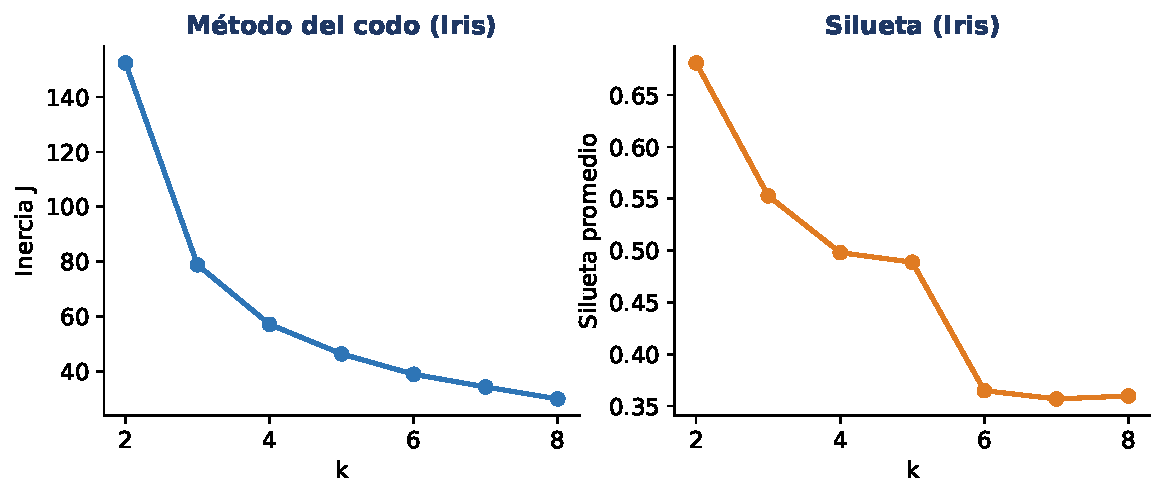
\includegraphics[width=0.62\textwidth]{iris_codo_silueta}\\
  \raggedright
  {\small El codo aparece entre $k=2$ y $k=3$. La silueta es máxima con $k=2$ (0.68) y baja a 0.55 con $k=3$.}
\end{frame}

\begin{frame}{Paso 2: ¿dos o tres grupos?}
  \begin{itemize}
    \item Los criterios numéricos sugieren $k=2$: una especie (setosa) está muy separada
          y las otras dos se traslapan.
    \item Con $k=3$ el codo todavía muestra una reducción importante de $J$ (de 152 a 79).
    \item Sabemos por el dominio que esperamos tres tipos de flor: elegimos $k=3$.
  \end{itemize}
  \vspace{6pt}
  \begin{alertblock}{Lección}
    La silueta mide qué tan separados quedan los grupos, no si corresponden a categorías reales.
    La elección de $k$ combina criterios numéricos y conocimiento del problema.
  \end{alertblock}
\end{frame}

\begin{frame}[fragile]{Paso 3: ajustar e interpretar los centros}
\begin{lstlisting}
km = KMeans(n_clusters=3, n_init=10, random_state=0).fit(X)
centros = pd.DataFrame(km.cluster_centers_, columns=X.columns)
print(centros.round(2)); print(np.bincount(km.labels_))
\end{lstlisting}
  \vspace{2pt}
  \centering
  \small
  \begin{tabular}{@{}lccccc@{}}
    \toprule
    \textbf{Grupo} & \textbf{Largo sépalo} & \textbf{Ancho sépalo} & \textbf{Largo pétalo} & \textbf{Ancho pétalo} & \textbf{Flores}\\
    \midrule
    A & 5.01 & 3.43 & 1.46 & 0.25 & 50 \\
    B & 5.90 & 2.75 & 4.39 & 1.43 & 62 \\
    C & 6.85 & 3.07 & 5.74 & 2.07 & 38 \\
    \bottomrule
  \end{tabular}\\[6pt]
  \raggedright
  \begin{itemize}
    \item Grupo A: pétalos pequeños y sépalos anchos.
    \item Grupos B y C: pétalos medianos y grandes, respectivamente.
  \end{itemize}
  {\small Los centros están en centímetros: se interpretan directamente como una flor ``típica'' de cada grupo.}
\end{frame}

\begin{frame}[fragile]{Paso 4: comparar con las especies}
\begin{lstlisting}
from sklearn.metrics import adjusted_rand_score
print(pd.crosstab(km.labels_, iris.target_names[especie]))
print(adjusted_rand_score(especie, km.labels_))   # 1 = coincidencia perfecta (S6)
\end{lstlisting}
  \begin{columns}[c]
    \column{0.58\textwidth}
    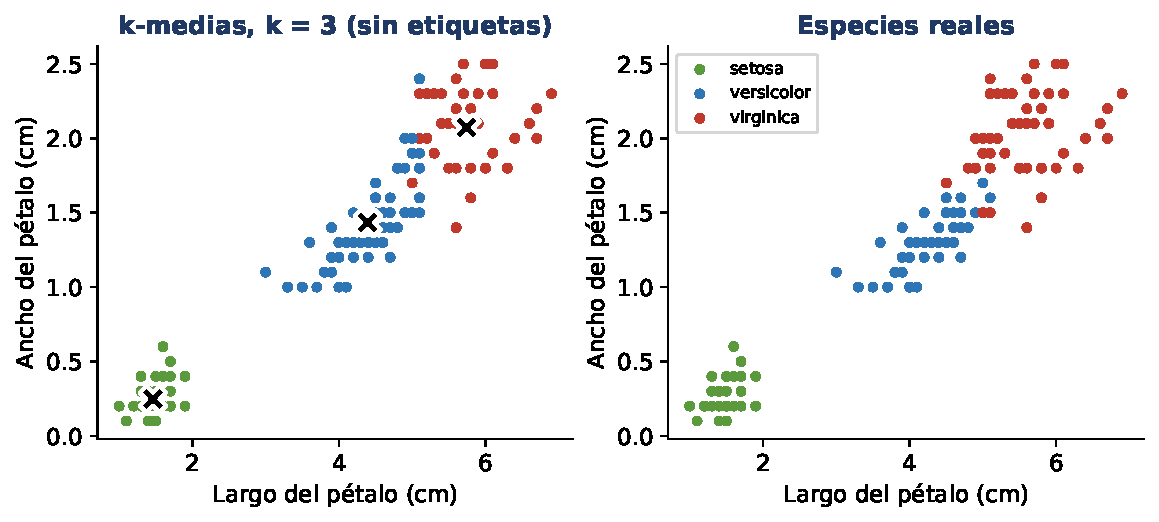
\includegraphics[width=\textwidth]{iris_resultado}
    \column{0.4\textwidth}
    \small
    \begin{tabular}{@{}lccc@{}}
      \toprule
      & \textbf{setosa} & \textbf{versic.} & \textbf{virgin.}\\
      \midrule
      A & 50 & 0 & 0 \\
      B & 0 & 48 & 14 \\
      C & 0 & 2 & 36 \\
      \bottomrule
    \end{tabular}\\[4pt]
    \begin{itemize}
      \item Setosa se recupera sin errores.
      \item 16 flores quedan en la frontera entre versicolor y virginica.
      \item Índice de Rand ajustado: 0.73.
    \end{itemize}
  \end{columns}
\end{frame}

\begin{frame}[fragile]{Paso 5: ¿conviene estandarizar?}
\begin{lstlisting}
from sklearn.pipeline import make_pipeline
from sklearn.preprocessing import StandardScaler

km_std = make_pipeline(StandardScaler(), KMeans(n_clusters=3, n_init=10, random_state=0))
etiquetas_std = km_std.fit_predict(X)
print(adjusted_rand_score(especie, etiquetas_std))
\end{lstlisting}
  \centering
  \small
  \begin{tabular}{@{}lcc@{}}
    \toprule
    \textbf{Datos ($k=3$)} & \textbf{Silueta} & \textbf{Rand ajustado}\\
    \midrule
    En centímetros & 0.55 & 0.73 \\
    Estandarizados & 0.46 & 0.62 \\
    \bottomrule
  \end{tabular}\\[6pt]
  \raggedright
  \begin{itemize}
    \item Aquí todas las variables tienen la misma unidad: estandarizar \alert{no es necesario}.
    \item Al estandarizar, el ancho del sépalo pesa lo mismo que los pétalos, que son más
          informativos, y el resultado empeora.
    \item Estandarizar es la regla cuando las unidades difieren (Sesión 1); no es automático.
  \end{itemize}
\end{frame}

\begin{frame}{Conclusiones del laboratorio}
  \begin{itemize}
    \item Sin usar la especie, k-medias descubre la estructura principal de Iris:
          un grupo bien separado y dos que se traslapan.
    \item Los criterios numéricos (silueta) sugieren $k=2$; el conocimiento del dominio lleva a $k=3$.
    \item Los centros, en las unidades originales, permiten describir cada grupo.
    \item Las decisiones de preprocesamiento cambian el resultado: deben justificarse.
    \item Las flores mal asignadas están en la frontera entre especies parecidas:
          k-medias asigna cada punto a un solo grupo, sin expresar incertidumbre
          (lo resolverán las mezclas gaussianas, Sesión 4).
  \end{itemize}
\end{frame}

% =====================================================================

\begin{frame}{Resumen}
  \begin{itemize}
    \item k-medias minimiza la \textbf{inercia}: suma de distancias cuadradas a la media de cada grupo.
    \item El algoritmo de Lloyd alterna asignación y actualización; siempre converge, pero a un \alert{mínimo local}.
    \item Usar \textbf{k-means++} y varios reinicios.
    \item Elegir $k$ con codo y silueta, y con criterio del problema.
    \item Supone grupos esféricos, convexos y de tamaño similar; es sensible a escala y atípicos.
  \end{itemize}
  \vspace{6pt}
  \begin{block}{Próxima sesión}
    Agrupamiento jerárquico: grupos anidados sin fijar $k$ de antemano.
  \end{block}
\end{frame}

\end{document}
